\documentclass[12pt,oneside,final]{siuethesis}
\usepackage{microtype} % (optional) for more beautiful typesetting
\usepackage{graphicx} 
\usepackage{hyperref} %makes links clickable
\hypersetup{colorlinks,citecolor=black,filecolor=black,linkcolor=blue,urlcolor=black} %good for electronic copy
\hypersetup{colorlinks,citecolor=black,filecolor=black,linkcolor=black,urlcolor=black}%required for paper graduate school copy
%\usepackage[alphabetic]{amsrefs} %required if using amsrefs, comment out if using bibtex
\usepackage{fixltx2e}
\usepackage{amsmath}
\usepackage{epsf}
%\usepackage{float}
\usepackage{caption}
\usepackage{subfig}
%\usepackage{subcaption}
\usepackage{listings}
\usepackage{rotating}
\usepackage{tabularx}
\usepackage{multirow}

%% controls numbering of theorems
%% this can be configured to your advisor's taste
\newtheorem{theorem}{Theorem}[chapter] %theorem number resets each chapter
\newtheorem{conclusion}[theorem]{Conclusion}
\newtheorem{condition}[theorem]{Condition}
%% conjectures, corollary, defn, etc. numbered sequentially from beginning of chapters
\newtheorem{conjecture}[theorem]{Conjecture} 
\newtheorem{corollary}[theorem]{Corollary}
\newtheorem{example}[theorem]{Example} 
\newtheorem{lemma}[theorem]{Lemma}
\newtheorem{proposition}[theorem]{Proposition}
\newtheorem{solution}[theorem]{Solution}
\theoremstyle{definition}
\newtheorem{definition}[theorem]{Definition}


\author{Bryan Orabutt}
\title{Design and Analysis of a Mult-Channel Discriminator Integrated Circuit for Use in Nuclear Physics Experiments}

%%\advisor{John Q.\ Faculty} %% or 
\advisor{Dr.}{George L. Engel}
\secondreader{Dr.}{Bradley Noble} %% or \secondreader{Dr.}{Karl Gauss}
\thirdreader{Dr.}{Timothy York}
%\fourthreader{Karl Gauss, Sr.}
%\fifthreader{Karl Gauss, Sr.}
%\secondadvisor{Karl Gauss} %if you haves two advisors (rare) then use this line also and pass the option `twoadvisors' to the class
%\abstracttext{Chairperson: The Honorable Jill Smith} %optional -- you can use this to override the text on the abstract page; the grad school default is built-in
\submitdate{August, 2018} %date the month/year submitted to grad school, use a comma between
\copyrightyear{2016} %optional, but required if copyrighted

%% all of these are optional; defaults are shown
\major{Electrical Engineering} 
\degree{Master of Science} %can be used to specify M.A., etc.
\highestdegree{Master of Science} %used if the author already has another graduate degree
\department{Electrical and Computer Engineering} 
%\departmentname{Department}
%\refname{REFERENCES} 

%\captionsetup{width=0.7\textwidth}

\begin{document}
\maketitle 

\frontmatter %signals single spacing/roman numeral pagination

\copyrightpage %optional


% ^^^^^^^^^^^^^^^^^^^^^
% ABSTRACT
% ^^^^^^^^^^^^^^^^^^^^^

\begin{abstract}

\par This thesis presents the design and simulation of a multichannel integrated circuit (IC) that will be used in nuclear physics experiments. The chip is being designed as a companion chip for another IC used in particle identification called PSD8C. The IC described in this thesis is used create precise timing pulses for starting time-to-voltage converters (TVCs) on the PSD8C. These timing pulses are created using a technique called constant fraction discrimination. Each of the sixteen channels in the IC contains a Nowlin circuit, leading edge discriminator, zero cross discriminator, and a one shot circuit to generate the output. \par The IC will support input pulse amplitudes between 20 mV and 2V both positive and negative, and input rise times between 3 nsec and 100 nsec. The IC will feature a programmable output pulse width between 50 nsec and 500 nsec. Most importantly the output pulse firing time variation will be independent of the input amplitude and rise time, having a time walk of only 1 nsec or less. The IC has been named CFD16C and the design presented is using the AMS-AG 0.35 micron NWELL process.
\end{abstract}


% ^^^^^^^^^^^^^^^^^^^^^^^^^^^^^^^^^^^^^^^
% ACKNOWLEDGEMNTS
% ^^^^^^^^^^^^^^^^^^^^^^^^^^^^^^^^^^^^^^^^


\begin{acknowledgements} 

\par I would first like to thank Dr. George Engel for being a continuous source of guidance through all my time working on this project. I would also like to thank Dr. Bradley Noble for encouraging me to investigate challenging problems and for being a source of guidance both in the classroom and out. I would also thank Dr. Timothy York for introducing me to IC design, without him I likely would never have gone to graduate school. I  would  like  to thank  Dr.  Lee  Sobotka  and  Mr.  Jon  Elson,  department  of  chemistry, Washington  University  Saint  Louis,  for  their  help  during  the  various  stages  of  this  project. My  special  thanks  to all of the  faculty  and  staff  of  ECE  department  for  their  direct  and  indirect support without which I simply could not have progressed with my work. Additionally, Dr. Gary Mayer of the Computer Science department has helped me expand knowledge beyond the skills learned in the classroom, and I am forever thankful. 
\par I would also like to thank the other graduate students I've been privileged to work with on this project as well. Pohan Wang, Prarthana Jani, Sneha Edula, and Anil Korkmaz and I all worked together to make CFD16C possible and they have helped make this project a pleasure to work on.
\par I would like to thank my friends Jack White, Jared Charter, Andrew Quirin, Nelly Sanchez, and Shana Mankouski for their support during all of my endeavours in graduate school. Finally I am forever grateful to my family for being a constant source of encouragement. My mother Marsha Orabutt, brother Sean Orabutt, and Vicki Kern who has been like a second mother to me, have all been there for me and I know I could not have come this far without them.

\end{acknowledgements}

\tableofcontents

\cleardoublepage %cause correct numbering of list of figures

\cleardoublepage

\listoffigures %print list of figures page

\cleardoublepage

\listoftables

\mainmatter %signals single spacing/arabic numeral paginations

% ^^^^^^^^^^^^^^^^^^^^^^^^^^^^^^^^^^^^^^^^^^^^^^^^^^^^^^^^^
%  CHAPTER 1
% ^^^^^^^^^^^^^^^^^^^^^^^^^^^^^^^^^^^^^^^^^^^^^^^^^^^^^^^^^

\chapter{INTRODUCTION}  %% chapter titles must be typed in all caps to conform with regulations

This chapter will introduce the reader to the field of radiation monitoring and describe how custom multi-channel integrated circuits is helping to re-shape this field.  The IC described in this thesis is the newest addition to the family of ICs which are being developed by the IC Design Research Laboratory at Southern Illinois University Edwardsville (SIUE in collaboration with researchers from the Nuclear Reactions Group at Washington University (WUSTL).

\section{Research Background}

The Integrated Circuits Design Research Laboratory at SIUE and the Nuclear Reactions Group at WUSTL have been working (since 2001) on a family of multi-channel custom integrated circuits.  The group became interested in developing a family of microchips for use in the detection and measurement of ionizing radiation because: (1) the need for high-density signal processing in the low- and intermediate-energy nuclear physics community is widespread, and (2) no commercial chips were identified that were capable of doing what the researchers wanted, and (3) the scientists deemed it necessary for the experimenter to be in the designer’s seat. The goal is to develop a ‘‘tool box’’ of circuits,
useful for researchers working with radioactive ion beams, which can be composed in different ways to meet the researchers’ evolving needs and desires.

 
The group’s first success was an analog shaped and peak sensing chip with on-board constant-fraction discriminators and
sparsified readout. This chip is designed for use with arrays of Si strip detectors of medium scale (with the number of channels ranging from a few hundred to a few thousand) and is known as Heavy-Ion Nuclear Physics–16 Channel (HINP16C). 

The second chip, christened Pulse Shape Discrimination–8 Channel(PSD8C), was designed to logically complement (in terms of detector types) the HINP16C chip. PSD8C performs pulse shape discrimination (PSD), and thus particle identification, if the time dependence of the light output of the scintillator depends on particle type. Moreover, PSD8C uses almost all the same supporting hardware as the HINP16C chip. Both ICs were fabricated in the ON-Semiconductor (formerly AMI) 0.5 mm n-well process (C5N), available through MOSIS (see \url{www.mosis.com}).

Talk about the block diagram of typical PSD system.

\begin{figure}[htbp!]
	\centering
 	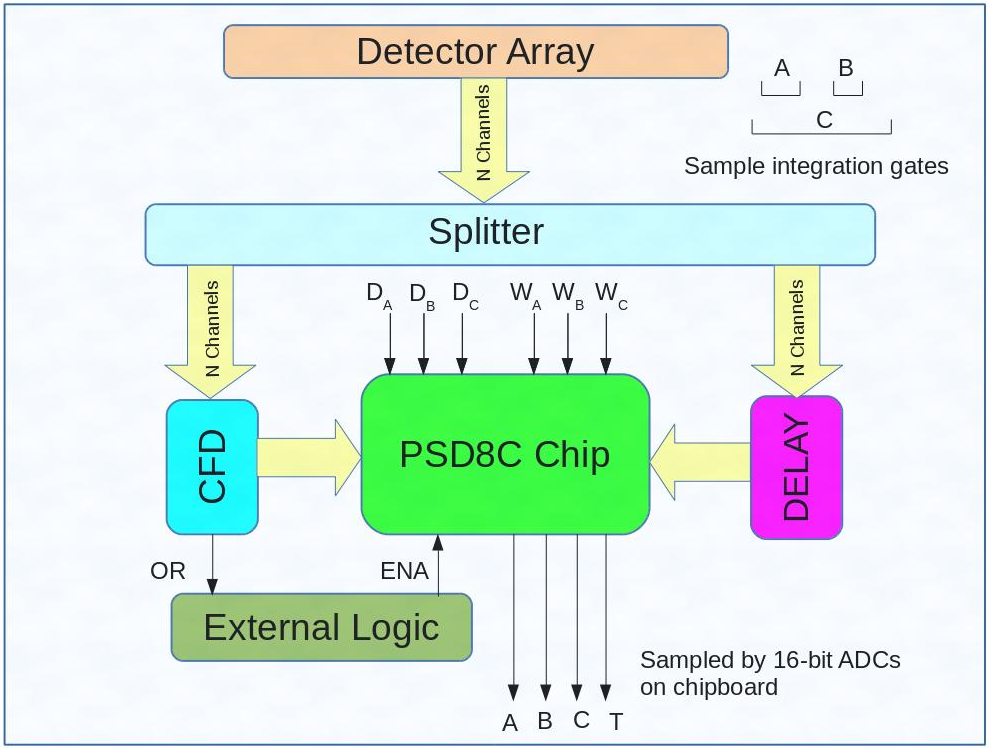
\includegraphics[scale=0.6,keepaspectratio=true]{./ch1_figures/PSD_block.png}
 	\caption{Block diagram of typical PSD system.}
 	\label{FIG:PSD_BLOCK}
\end{figure}


\section{PSD8C IC}

Our PSD8C chip greatly simplifies the pulse-processing electronics needed for large arrays of scintillation detectors. Each channel(see Figure~\ref{FIG:PSD_CHANNEL}) possesses 3 sub-channels. The sub-channels are referred to as A, B, and C. A sub-channel consists of an integrator and a gate generator. External control voltages (DX, WX) determine the gate delay and the gate width. The structure of a single PSD8C sub-channel is illustrated in Figure~\ref{FIG:PSD_SUB_CHANNEL}. Because PSD8C employs (user-controlled) multi-region charge integration, particle identification is incorporated into the basic design. Each channel on the chip also contains a TVC that provides relative time information. The pulse height integrals and the relative time are all stored on capacitors and are either reset, after a user-controlled time, or sequentially read out if acquisition of the event is desired (in a manner similar to that of HINP16C). 

\begin{figure}[htbp!]
	\centering
 	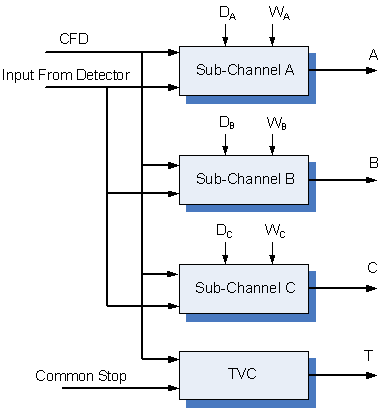
\includegraphics[scale=1.0,keepaspectratio=true]{./ch1_figures/PSD_channel.png}
 	\caption{PSD Channel}
 	\label{FIG:PSD_CHANNEL}
\end{figure}


\begin{figure}[htbp!]
	\centering
 	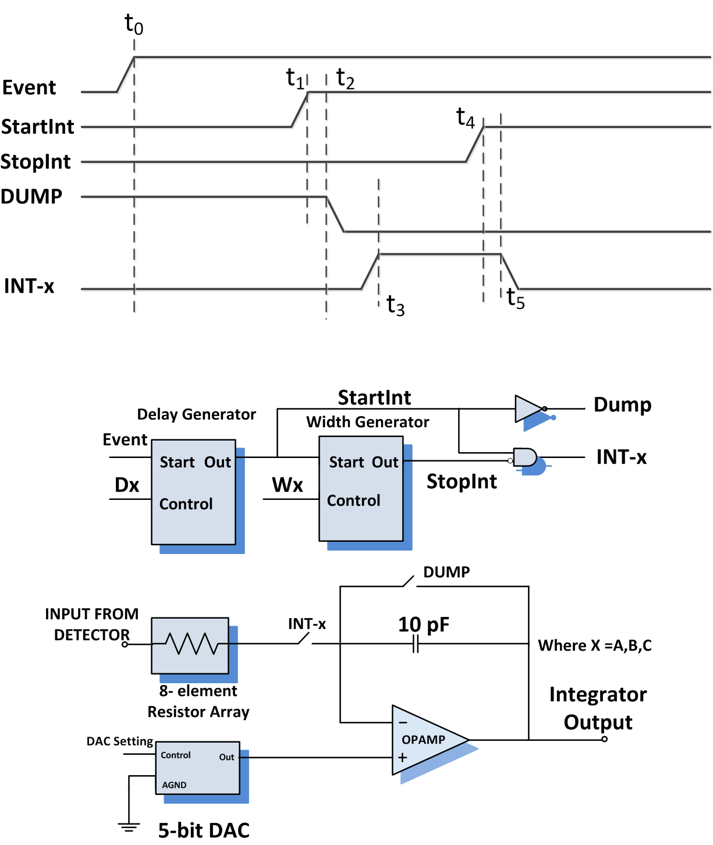
\includegraphics[scale=1.3,keepaspectratio=true]{./ch1_figures/PSD_sub_channel.png}
 	\caption{PSD Sub-channel.}
 	\label{FIG:PSD_SUB_CHANNEL}
\end{figure}

Features of the first generation PSD8C (Rev. 1) chip include:
\begin{itemize}
\item
eight independent channels per IC;
\item
on-chip data sparsification;
\item
each channel automatically resets itself after a user programmable delay time;
\item
three (3) integration regions each with: (a) independent
control of time offset (beginning), (b) width (ending) of the
integration window, and (c) a menu of eight (8) charging rates;
\item
each channel possesses a TVC with two time ranges: 500 ns and 2 ms;
\item
three triggering modes;
\item
fast logical OR-gate and an analog multiplicity output to aid in
trigger decisions;
\item
two power modes to facilitate use with fast and slow detectors
and to thus allow for a more modest power budget for the
latter; 
\item
and CFD circuits are not on-chip so as to provide greater flexibility.
\end{itemize}

PSD8C is described in detail in \cite{PROCTOR} and \cite{HALL}. PSD8C is 2.25 by 5.7 $mm^2$ and is packaged in a 14 by 14 $mm^2$, 128 lead thin quad flat pack. Power consumption is 65 mW (low-bias mode)and 150 mW (high-bias mode). The cost per channel is 25.
A second version (Rev. 2) of PSD8C was submitted for fabrication in May 2010. Rev. 2 attempts to correct several minor
problems. First, the TVC circuit could inadvertently be re-started. In Rev. 2, once the rising edge of the ‘‘common stop’’ signal is detected, the TVC cannot re-start until the channel is reset. Second, undesirable temperature dependence (1 ns/C) in the TVC circuit was identified and traced to the local channel buffer. The buffer was redesigned, and the TVC temperature sensitivity has been greatly reduced (5 ps/C in the 500 ns mode, 40 ps/C in the 2 ms mode). Third, some TVC crosstalk issues were identified and remedied. Fourth, additional shielding was added to the integrator circuits. Finally, at the system level, the chip-boards (printed-circuit boards) were redesigned to include on-board ADCs (one for each of the chip’s analog output pulse trains).

(Still need to talk about enhancements that were made on PSD4)


\section{Need for an Integrated Circuit}

While not including the timing circuits on PSD made it more flexible, those circuits are needed.  Currently, a large complex board with many ICs produce the timing signals required by the PSD chip. This thesis describes the design of multi-channel integrated circuit which can generate the timing signals for a pair of PSD chips.

\begin{figure}[htbp!]
	\centering
 	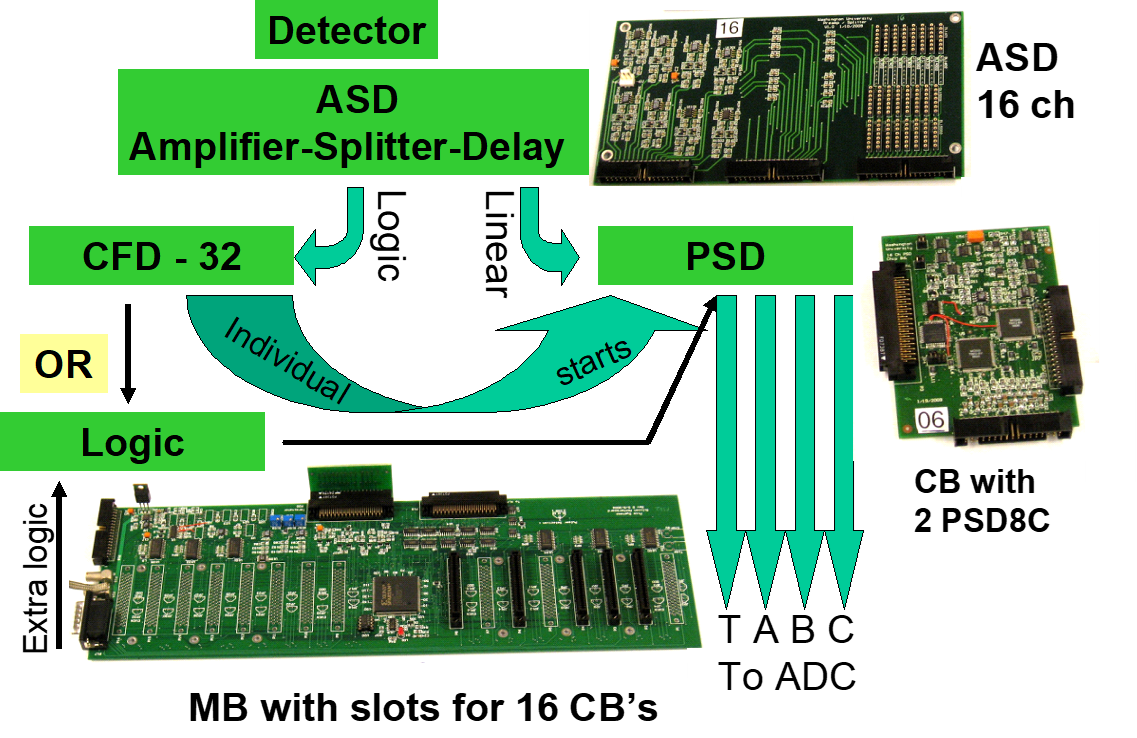
\includegraphics[scale=0.8,keepaspectratio=true]{./ch1_figures/PSD_system.png}
 	\caption{PSD system using board-level CFD electronics}
 	\label{FIG:PSD_SYSTEM}
\end{figure}



\section{Sample Applications}

To focus the reader’s attention on what would be possible with the PSD chip complemented by the CFD chip described in this thesis, consider a highly granular discrete element array for neutron detection using the recently developed inorganic [9] and plastic [11] scintillators with PSD. Such a large array would open the n-rich side up to the kind of high-precision work the Washington University group has done on the p-rich side. (The existing work on the neutron-rich side, done at high energy and with detectors such as MONA-LISA [12], while providing provocative data on such cases as 16Be [13] and 26O [14], sufferer for poor statistics and, compared to the proton-rich side, poor resolution.) An array to be deployed at low (reaccelerated beam) energies with thousands of optically isolated PSD elements made from the new generation of plastics, would revolutionize the study of multiple n-decay from what are generally high-isospin states. (The problem of detector-to-detector scattering cross-talk can also be improved with discrete pixilated – rather than using large bars – by corrugating the detectors in the same way as the conventional discrete array DEMON has [15].  

While we are enamored with the above idea, it is premature to propose such an array before the ground-work for scalable timing electronics, as we describe in this thesis, is successfully completed. (In fact the coupling of the scintillator – from Eljen – to the new blue sensitive SiPMs – from SensL – is simple compared to the development of the scalable electronics.) To this end however, we plan to develop a circuit board using the PSD and CFD chips to process signals from the new generation of PSD-capable plastic scintillators [11]. 

The CFD chip described herein with its programmable Nowlin cirucit will allow the WUSTL Nuclear Rewactions Gropup to work with variety of scintillators (LaBr:Ce to CsI:Tl or :Na to standard plastics and, for what might be the most interesting untapped opportunity, the new class of PSD capable plastics [11)].  


\section{Object and Scope of Work} 

\par The object of this thesis work was to create a multichannel integrated circuit capable of constant fraction discrimination. This thesis is composed of five chapters. The system level architecture is presented in Chapter 2. Chapter 3 describes the circuit level design of the many sub-circuits that compose the CFD16C. Chapter 4 details the simulated performance of the CFD16C to show that it performs within the intended design specification. Finally Chapter 5 provides a summary, conclusions, and details future work to be done on the CFD16C.

% ^^^^^^^^^^^^^^^^^^^^^^^^^^^^^^^^^^^^^^^^^^^^^^^^^^^^^^^^^
%  CHAPTER 2
% ^^^^^^^^^^^^^^^^^^^^^^^^^^^^^^^^^^^^^^^^^^^^^^^^^^^^^^^^^


\chapter{SYSTEM ARCHITECTURE}

This chapter will attempt to describe the CFD16C integrated circuit at the system-level.  We will start with a detailed list of system requirements and then will describe the high-level architecture of the IC.

\section{System Specifications}
The success of our group over the past 20 years lies in the fact that in the close working relationship that the IC Design Research Laboratory at Southern Illinois University Edwardsville (SIUE) has had with the Nuclear Reactions Group at Washington University in St. Louis(WUSTL) led by Dr. Lee Sobotka.  The IC group here at SIUE and the Nuclear Reactions Group at WUSTL, after lengthy discussions, drafted the following specifications for the IC described here in this thesis.

\begin{itemize}
\item
The IC should support 16 detectors.
\item
It should support analog pulses of both polarities (relative to analog signal ground).
\item
It should accommodate analog exponentially shaped pulses with risetime constants ranging from 3 nsec to 100 nsec.
\item
It exhibit "excellent" walk and jitter characteristics for input pulse amplitudes ranging from 20 mV to 2 V. The adjective "excellent" will be quantified in a later chapter of this thesis.
\item
Pulse repetition rates up to 1 KHz must be accommodated.
\item
The discriminator in each of the 16 channels should be of the constant fraction type (CFD). In CFD discriminators an attenuated version of the input is subtracted from a delayed version of input waveform and the time at which the difference between the two is equal to zero is used to mark the pulse arrival time. This results in output timing signals independent of pulse amplitude.
\item
Each channel should have a leading-edge threshold.
\item
While the chip must support signals with risetime constants ranging from 3 nsec to 100 nsec, performance will be optimized for the shorter time constants. 
\item
The output pulse width from a channel should be programmable.
\item
The IC should operate from a single 3.3 Volt supply.
\item
Power consumption of the 16 channel IC should not exceed 350 mW \emph{i.e.} 20 mW per channel with 30 mW budgeted for the circuits common to all channels. 
\item
The IC is not to occupy an area greater than roughly 2 mm x 3 mm.  The chip should be packaged in a 64-pin plastic package.  

\end{itemize} 

\section{Features}

\section{System-Level Description}

\section{Chip Pinout}

% ^^^^^^^^^^^^^^^^^^^^^^^^^^^^^^^^^^^^^^^^^^^^^^^^^^^^^^^^^
%  CHAPTER 3
% ^^^^^^^^^^^^^^^^^^^^^^^^^^^^^^^^^^^^^^^^^^^^^^^^^^^^^^^^^


\chapter{ELECTRICAL LEVEL DESIGN}

\section{Fabrication Process}

The IC described in this thesis will be fabricated in the AMS-AG 0.35 micron NWELL process.  The process supports two poly and 4 metal layers. Double poly capacitors, BJTs, and a high-resistance layer are all available to the designer. NFET device properties are given in Table~\ref{TBL:NMOS_PARMS} while PFET device properties are availabe in Table~\ref{TBL:PMOS_PARMS}.

% NFET device properties

\begin{table} [htbp!]
\begin{center}
\begin{tabular}{| l | c | c |}
\hline 
Threshold Voltage & $V_{TN}$ & 0.5 V \\ 
\hline 
Transconductance Parameter & $K_{PN}$  &  170 $\frac{\mu A}{V^2}$ \\ 
\hline 
Bulk Modulation Factor & $\gamma_{N}$  &  0.6 $V^{\frac{1}{2}}$ \\ 
\hline 
Early Voltage per Unit Length & $V_{EN}$  &  21.1 $\frac{V}{\mu m}$ \\ 
\hline 
Gate Oxide Thickness & $t_{ox}$  &  7.6 nm \\ 
\hline 
Gate Oxide Capacitance per Unit Area & $C_{ox}$  & 4.5 $\frac{fF}{\mu m^2}$ \\ 
\hline 
Threshold Voltage Matching Coefficient & $A_{VTN}$  &  9.4 mV $\cdot$ $\mu m$ \\ 
\hline 
Transconductance Matching Coefficient & $A_{KPN}$  &  0.7 \% $\cdot$ $\mu m$ \\ 
\hline 
\end{tabular} 
\end{center}
\caption{NMOS Parameters}
\label{TBL:NMOS_PARMS}
\end{table}

% PFET device properties
 
\begin{table} [htbp!]
\begin{center}
\begin{tabular}{| l | c | c |}
\hline 
Threshold Voltage & $V_{TP}$ & -0.7 V \\ 
\hline 
Transconductance Parameter & $K_{PP}$  &  60 $\frac{\mu A}{V^2}$ \\ 
\hline 
Bulk Modulation Factor & $\gamma_{P}$  &  0.4 $V^{\frac{1}{2}}$ \\ 
\hline 
Early Voltage per Unit Length & $V_{EP}$  &  17.7 $\frac{V}{\mu m}$ \\ 
\hline 
Gate Oxide Thickness & $t_{ox}$  &  7.6 nm \\ 
\hline 
Gate Oxide Capacitance per Unit Area & $C_{ox}$  &  4.5 $\frac{fF}{\mu m^2}$ \\ 
\hline 
Threshold Voltage Matching Coefficient & $A_{VTP}$  &  14.5 mV $\cdot$ $\mu m$ \\ 
\hline 
Transconductance Matching Coefficient & $A_{KPP}$  &  1.0 \% $\cdot$ $\mu m$ \\ 
\hline 
\end{tabular} 
\end{center}
\caption{PMOS Parameters}
\label{TBL:PMOS_PARMS}
\end{table}

% DESCRIPTION OF COMMON CHANNEL

\section{Common Channel}
\par The CFD16C is composed of sixteen signal channels and a single larger common channel. As the name implies, the common channel contains configuration and biasing circuitry that is common to all of the signal channels. These include a power on reset circuit, signal ground generator, bandgap reference, and bias current generators.

\subsection{Configuration registers}
\par There are three registers in the common channel as well as one in each of the signal channels. Each register can be individually selected by providing an appropriate address and mode as shown in Table~\ref{tab:registers}. Address and mode are registered on the positive edge of the input STB signal, while data is registered on the falling edge. All registers in the common channel are selected with an address of 0000. 

\begin{table}[htbp!]
 \centering
 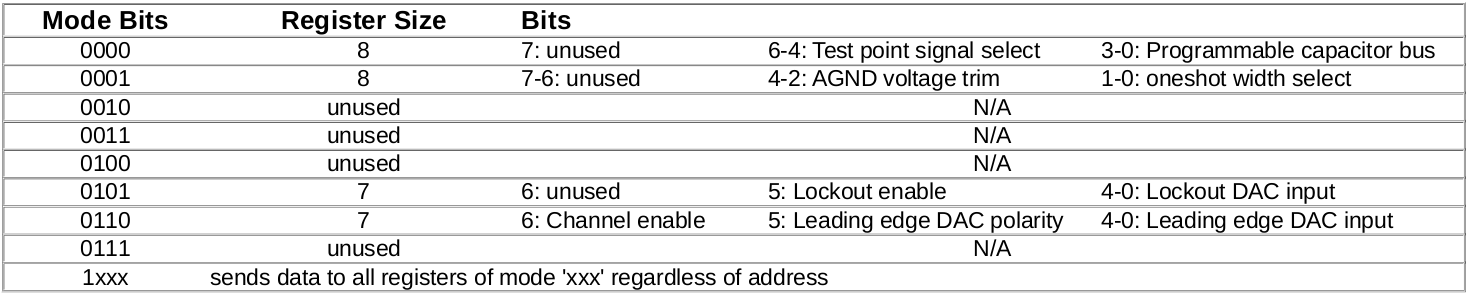
\includegraphics[scale=.3,keepaspectratio=true]{../data/modes.png}
 \caption{Register mode usage.}
 \label{tab:registers}
\end{table}


\subsection{Power on reset circuit}
\par A power on reset circuit is used to start the PTAT bias current generator circuit. When power is applied to the CFD16C, the power on reset (POR) circuit generates a single low active reset pulse. This reset pulse is guaranteed to be at least 2 $\mu sec$ long. This long reset pulse guarantees that the PTAT current generator will start correctly and provide an 11.5 $\mu A$ bias current.

\subsection{Signal ground generator}
\par In each of the signal channels the analog input circuitry is all referenced to a seperate signal ground. This signal ground, called AGND, must be at a potential half way between AVDD and AVSS. The signal ground generator circuit can be trimmed to a specific voltage using three trim bits. The signal ground generator has a nominal reference voltage of 1.63 V and can be trimmed by $\pm 250$ mV.

\subsection{Bandgap voltage reference}
\par The bandgap voltage reference used in this design was copied from PSD8C as a known working solution. A bandgap voltage reference is used to provide a 1.2 V reference point that is independent of temperature or power supply noise. The bandgap voltage is created by generating a PTAT series resistor and a diode-connected parasitic bipolar PNP transistor \cite{ALLEN}. The PTAT current has a positive temperature coefficient while the PNP transistor has a negative temperature coefficient creating a nodal voltage with a temperature coefficient of only -87 $\frac{\mu V}{C}$.
\par This bandgap topology produces an output voltage of $\approx 1.2 V$ with near zero temperature independence. The design was pulled from an analog cells library provided by AMS and is a known working and manufactured component.

\subsection{PTAT current reference}

\subsection{Zero-tempco current reference}
\par In order to function correctly, some of the circuitry in the signal channel needs to be biased with a current that has no temperature dependence. This zero temperature coefficient (ZTC) current was generated using an opamp circuit shown in Figure~\ref{fig:ztc}. In this circuit, the temperature independent bandgap voltage is applied to the inverting terminal of an opamp. The output of the opamp connects to the gate of a PFET whose drain is connected to a zero temperature coefficient 100 k$\Omega$ resistor. A feedback connection to the non-inverting terminal of the opamp is made to the drain of the PFET as well. 
\par Because of this feedback connection, the opamp will drive the gate of the PFET to a voltage that ensures there is no potential difference between the inverting and non-inverting terminals of the opamp. This means the voltage drop across the ZTC resistor has to be equal to the bandgap voltage and so the current through the PFET has to be 12 $\mu$A.
\begin{figure}[htbp!]
\centering
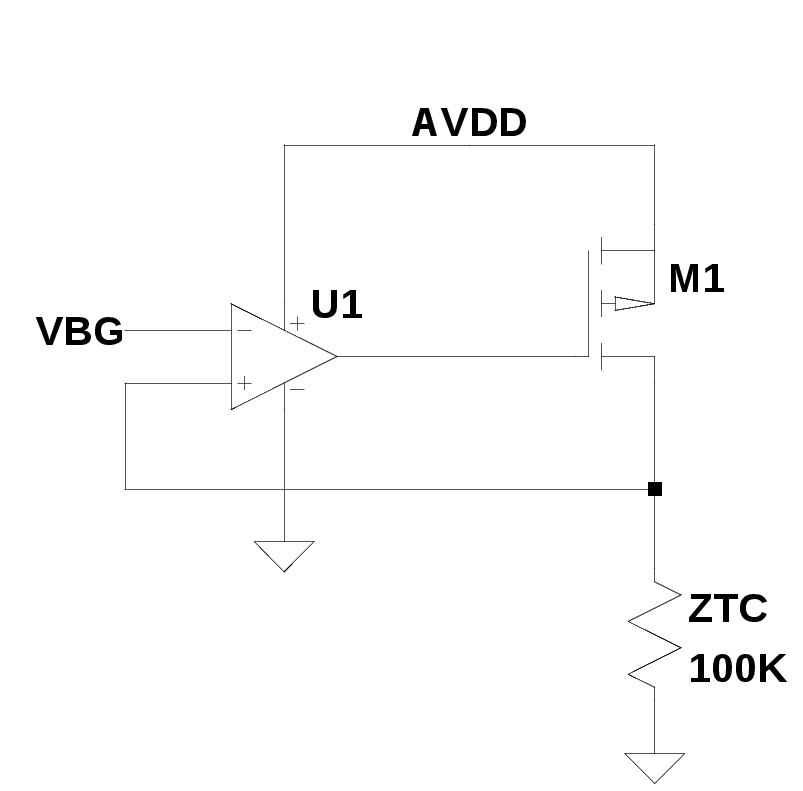
\includegraphics[scale=.25,keepaspectratio=true]{../LTspice_Drawings/ztc_iref/circuit.png} 
\caption{Zero temperature coefficient current generator.}
\label{fig:ztc}
\end{figure}
\par The ZTC resistor is made from a resistor with positive temperature coefficient (rpoly2), and one that has a negative temperature coefficient (rpolyh). The ratio to achieve temperature independence in this process is $\approx$0.56 rpoly2 to 0.44 rpolyh. Since a 12 $\mu$A ZTC current is desired, a 100 k$\Omega$ resistor was made using a 56 k$\Omega$ rpoly2 resistor and a 44 k$\Omega$ rpolyh resistor. This ZTC current is replicated using 17 current mirrors to provide one for each channel, as well as one for the lockout DAC in the common channel. The ZTC currents are used to give the DAC circuits an output that doesnt depend on temperature. 
\subsection{Lockout DAC}

\subsection{Multiplicity output buffer}


% DESCRIPTION OF SIGNAL CHANNEL

\section{Signal Channel}

\subsection{Programmable Nowlin circuit}

\subsection{Leading-edge detector}

\subsection{Zero-cross detector}


\subsection{Output one-shot with lockout features}



% ^^^^^^^^^^^^^^^^^^^^^^^^^^^^^^^^^^^^^^^^^^^^^^^^^^^^^^^^^
%  CHAPTER 4
% ^^^^^^^^^^^^^^^^^^^^^^^^^^^^^^^^^^^^^^^^^^^^^^^^^^^^^^^^^


\chapter{SIMULATION RESULTS}

\section{Verification of Circuits in Common Channel}

\section{Walk Characteristics of CFD Circuitt}

\section{Jitter Performance}

\section{Verification of One-Shot}

\section{Performance Characterization of DAC}

\section{Chip-Level Verification}


% ^^^^^^^^^^^^^^^^^^^^^^^^^^^^^^^^^^^^^^^^^^^^^^^^^^^^^^^^^
%  CHAPTER 5
% ^^^^^^^^^^^^^^^^^^^^^^^^^^^^^^^^^^^^^^^^^^^^^^^^^^^^^^^^^


\chapter{SUMMARY, COMCLUSIONS, AND FUTURE WORK}

\section{Summary}


\section{Conclusions}

\section{Future Work}

\references %single spacing / arabic numeral paginations, adds "REFERENCES" to table of contents

%%%% for bibtex

%If you want to use bibtex  use the following lines, where your .bib file is called 'yourbib.bib'

\bibliographystyle{apalike}
\bibliography{./Orabutt_Thesis.bib}

% If you have only a single appendix, do it this way.

\multipleappendices
\lstset{
         language=C,
         basicstyle=\scriptsize\ttfamily,
         emptylines=0, 
         lineskip=1pt,
         %numbers=left,            
         numberstyle=\tiny,         
         stepnumber=2,              
         numbersep=5pt,             
         tabsize=3,                
         extendedchars=true,       
         breaklines=true,            
         commentstyle=\color{blue},
         keywordstyle=\color{red},
            frame=b,         
 %        keywordstyle=[1]\textbf,    
 %        keywordstyle=[2]\textbf,    
 %        keywordstyle=[3]\textbf,  
 %        keywordstyle=[4]\textbf,   \
         stringstyle=\scriptsize\color{green}\ttfamily, 
         showspaces=false,         
         showtabs=false,            
%         xleftmargin=17pt,
%         framexleftmargin=17pt,
%         framexrightmargin=5pt,
%         framexbottommargin=4pt,
         %backgroundcolor=\color{lightgray},
         showstringspaces=false           
 }


\end{document}
